\chapter{Validierung}
%Überprüfen der Thesen
%    Szenarien mit erwarteten Ergebnissen vergleichen
%    Ergebnisse über Prototyp bestätigen
    
Um bewerten zu können, ob das entwickelte Programm den in Kapitel 4 genannten Anforderungen entspricht, wird in diesem Kapitel zur Validierung ein virtualisiertes Labor aufgebaut, das einen virtuellen \ac{IoT}-Client, einen virtuellen Broker und den Proxy bereitstellt.

%Szenario, was mit dem Labor versucht wird zu erreichen.
Das Labor bildet die Kommunikation zwischen einem Sensor, welcher sich in der Glühbirne im Wohnzimmer des Nutzer befindet, und dem Broker des Herstellers ab. Der Sensor, im weiteren \emph{Client} genannt, stellt dem Broker jede Sekunde den aktuelle Status zur Verfügung. Der Broker hingegen erwartet den Status eines Clients und veröffentlicht diesen für andere externe Clients.

\begin{figure}[h]%h=direkt danach t=top b=bottom
    \centering
    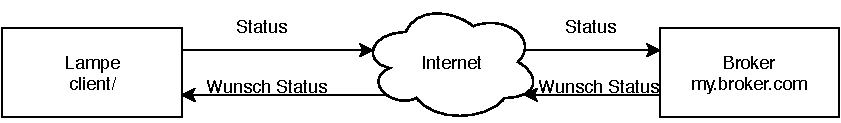
\includegraphics[width=14cm]{tex/bilder/6_validierung/Szenario.pdf}
    \captionof{figure}{Darstellung des Szenarios}
    \label{fig:darstellung-szenario}
\end{figure}

\section{Laboraufbau} \label{Laboraufbau}
    %Warum Virtualisierung/ Virtualisierte Umgebung
    Das Labor wird mithilfe der Virtualisierungslösung \emph{ESXi} %\cite{https://www.vmware.com/de/products/esxi-and-esx.html}
    der Firma \emph{VMware} umgesetzt. Dadurch, dass alle Systeme und Applikationen in sogenannten virtuellen Maschinen laufen, sind sie, obwohl sie auf dem gleichen physikalischen Gerät (Server) laufen können, voneinander unabhängig. Das bedeutet, dass ganze Systeme abgeschottet und auf virtuellen Festplatten (sog. \emph{\acp{VMDK}}) gespeichert und somit auch sehr einfach gesichert oder untereinander ausgetauscht werden können. Durch die dynamische Verteilung von zum Beispiel \ac{CPU} oder RAM ist ebenfalls eine effektivere Nutzung von Hardwareressourcen möglich. Damit wird nur ein Server oder leistungsfähiger Computer benötigt um ganze Systemlandschaften und Netzwerke abzubilden. Des Weiteren ermöglicht es auch, die hier durchgeführten Tests und somit Ergebnisse in der gleichen Umgebung durch die Bereitstellung der Dateien nachvollziehen zu können, ohne selbst Arbeit und Zeit in den Aufbau derselben Systeme investieren zu müssen.
    %Warum mit ESXI
    \emph{ESXi} wurde als Lösung gewählt, da bereits Wissen und Erfahrung im Umgang mit der Lösung vorhanden war. Zusätzlich stand ein Server mit benötigter Leistung bereits zur Verfügung wodurch das Aufsetzen und Konfigurieren eines solchen oder ähnlichen Produkts nicht mehr nötig war.
    
    Die folgenden Voraussetzungen sind notwendig um das Programm ausführen zu können:
    \begin{itemize}
        \item Betriebssystem: ab Windows 7, Linux mit Mono
        \item Abhängigkeiten: .NET Framework v4.6.1, Mono ab 4.2.0.X
        \item Speicher: 50 \ac{MB} frei
        \item RAM: 100 \ac{MB} frei
        \item Prozessor: 2 virtuelle Kerne  mit 2,0 Ghz
        \item Netzwerkkarte: Ja
    \end{itemize}
    
    \subsection{Virtualisierung der Geräte}
    Die in diesem Szenario enthaltenen Systeme sind die Folgenden:
    \begin{table}[h]
        \centering
        \begin{tabular}{c|c|c|c}
            Name & Client & Broker & Proxy \\ \hline
            OS & Debian 9 & Debian 9 & Microsoft Windows 10 \\
            CPU & 1 vCPUs & 1 vCPUs & 4 vCPUs \\
            RAM & 512 \ac{MB} & 512 \ac{MB} & 8 GB \\
            HDD & 5 GB & 5 GB & 50 GB \\
        \end{tabular}
        \caption{Ressourcen der Virtuelle Maschinen}
        \label{tab:ressourcenverteilung}
    \end{table}
    
    Der Client verwendet folgende Software:
    \begin{itemize}
        \item Python 2.7.X
        \item pip-Paket: paho-mqtt
    \end{itemize}
            
    Der Broker arbeitet mithilfe folgender Software:
    \begin{itemize}
        \item Python 3.X, Python3-pip
        \item pip-Paket: hbmqtt
    \end{itemize}
            
    Das Proxy-System, welches die Kommunikation überwacht, benötigt zum Ausführen der Proxy-Anwendung folgende Software:
    \begin{itemize}
        \item Microsoft Visual C++ 2008
        \item Microsoft Visual C++ 2017
        \item .NET Framework 4.6.1\footnote{Dadurch, dass das .NET Framework Bibliotheken, Kompiler und Laufzeitumgebungen bereitstellt, ist es notwendig diese in der oben genannten Version zu installieren um in diesem Projekt verwendete Funktionen nutzen zu können und das Programm zu kompilieren.}
    \end{itemize}
    
    \subsection{Netzwerk}
    Es werden Netzwerke verwendet in denen sich alle Geräte befinden. 
    Das erste Netzwerk beinhaltet den Audit PC, die Proxy Anwendung und den virtuellen Broker sowie die Firewall als Schnittstelle zum zweiten Netzwerk.
    Die Firewall spannt ein \ac{VLAN} auf, in dem sich der Client befindet. Mittels Portweiterleitung\footnote{Pakete, die an einen spezifizierten Port beinhalten, werden an ein festgelegte Adresse weitergeleitet.} leitet es den Datenverkehr des Clients zum Proxy um. %TODO FRAGEN OB QUELLE NOTWENDIG
    
    \begin{figure}[h]%h=direkt danach t=top b=bottom
        \centering
        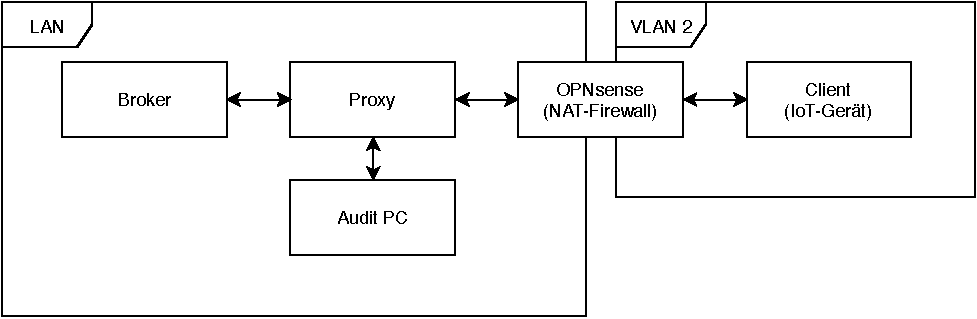
\includegraphics[width=14cm]{tex/bilder/6_validierung/Netzwerkdiagramm.pdf}
        \captionof{figure}{Darstellung des virtuellen Netzwerks}
        \label{fig:virtuelles_netzwerk}
    \end{figure}
    
    \subsection{Konfiguration der Software} \label{KonfigurationDerSoftware}
    %Konfiguration
    Das Projekt ist im Standard auf Prozessoren mit x86-Befehlssatz ausgerichtet, kann allerdings bei Bedarf auch auf Prozessoren mit x64-Befehlssatz durch Änderung der entsprechenden Einstellung in Visual Studio geändert werden.
    Eine Unterstützung für weitere Architekturen ist durch die Installation plattformübergreifender Implementierungen von Mono und Python möglich. Auch muss hierzu in Visual Studio die Zielarchitektur auf "Any CPU" gesetzt werden. 
    Zusätzlich ist zur Ausführung der Anwendung ein privilegierter Account erforderlich, um die Berichtigung für Zugriff auf die erforderlichen Ports zu erhalten.
    
    Es werden Port 1883 für die Kommunikation über das \ac{MQTT}-Protokoll und Port 80 für die \ac{REST} Schnittstelle und einen Webserver, der die Weboberfläche bereitstellt, benötigt.
    Der Proxy ist ausschließlich über die Adresse \glqq 127.0.0.1\grqq{} oder \glqq localhost\grqq{} erreichbar, da keine Benutzerauthentifizierung implementiert wurde. Im lokalen Netz oder bei Bereitstellung über eine öffentlich erreichbare Adresse, kann eine unberechtigte Verwendung nicht ausgeschlossen werden. Daher wird dies auch nicht empfohlen. Sofern jedoch die Notwendigkeit bestehen sollte, ist es möglich die Adresse im Quellcode durch die lokale IP-Adresse des Gerätes, auf dem der Proxy ausgeführt wird, auszutauschen, um eine parallele oder externe Verwendung zu ermöglichen.

    Für den Broker wird eine Konfigurationsdatei, wie in Listing \ref{fig:broker_config} zu sehen, angelegt. Diese definiert unter Anderem, wie viele Verbindungen akzeptiert werden und auf welchem Interface gelauscht wird. Anschließend wird noch die Authentifizierung deaktiviert und mithilfe von einem Plugin werden \emph{Topics} von eingehenden Nachrichten automatisch erzeugt. 
    \begin{figure}[h]
        \begin{lstlisting}
            listeners:
              default:
                max-connections: 5000
                bind: 0.0.0.0:1883
                type: tcp
            auth:
              allow-anonymous: true
            topic-check:
              enabled: True
            plugins:
              - topic_taboo
        \end{lstlisting}
        \captionof{figure}{Broker Konfiguration}
        \label{fig:broker_config}
    \end{figure}

\section{Ausführung und Bewertung}
Auf Abbildung \ref{fig:client_messages} ist der erstellte virtuelle Client zu sehen, welcher Nachrichten über den Proxy an den Broker schickt.
%Was für Nachrichten
Nach dem erfolgreichen Abonnieren des \emph{Topics}, sendet der virtuelle Client jede Sekunde eine Nachrichten mit dem aktuellen Status an den Broker. Kurz darauf veröffentlicht der Broker diese Nachricht in dem abonnierten \emph{Topic}. Aus diesem Grund erhält der Client anschließend dieselbe Nachricht wieder zurück. Abhängig vom Szenario muss der Client nicht an seinen Veröffentlichungen interessiert sein und kann auch andere \emph{Topics} \emph{"subscriben"} (abonnieren).
\begin{figure}[!h]%h=direkt danach t=top b=bottom
    \centering
    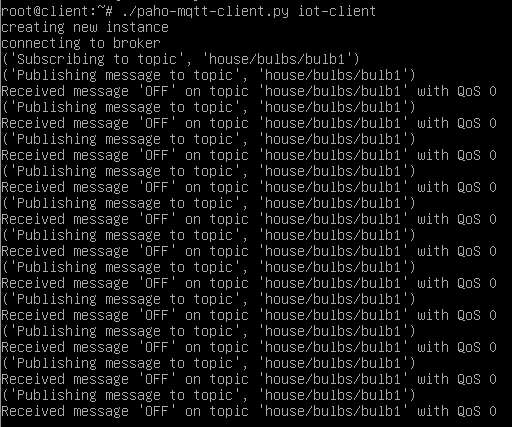
\includegraphics[width=10cm]{tex/bilder/6_validierung/ClientMessages.png}
    \captionof{figure}{Darstellung des gesendeten Nachrichten vom Client}
    \label{fig:client_messages}
\end{figure}

In Abbildung \ref{fig:broker_connections} ist die Initialisierung des Brokers zu sehen. Er wird mithilfe einer Konfigurationsdatei gestartet (siehe \ref{KonfigurationDerSoftware}). Anschließend wird angezeigt, dass erst eine und danach eine zweite Verbindung zum Broker hergestellt wurde. Diese Verbindungen werden allerdings nicht mit dem virtuellen Client, sondern den Clients des Brokers aufgebaut.
\begin{figure}[!h]%h=direkt danach t=top b=bottom
    \centering
    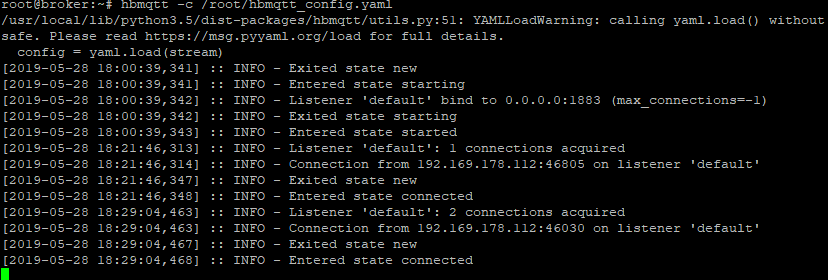
\includegraphics[width=14cm]{tex/bilder/6_validierung/BrokerConnections.png}
    \captionof{figure}{Darstellung der Client-Verbindungen beim Broker}
    \label{fig:broker_connections}
\end{figure}

Der Proxy zeigt, wie Abbildung \ref{fig:proxy_messages} zu entnehmen ist, beim Erhalt einer Nachricht, vom virtuellen Client (\ac{IoT}-Gerät), sowie vom Proxy Client (\emph{ClientIn}), deren Inhalt an.
Darüber hinaus, zeigt er auch weitere Aktionen des \emph{ClientManagers} und der virtuellen Client an.
Mithilfe der Nachrichten lassen sich der Ablauf des Programms und etwaige Fehler nachvollziehen. Diese Ausgabe kostet jedoch vergleichsweise viel Leistung, woraus die in \ref{Laboraufbau} aufgeführten Systemanforderungen resultieren. 
\begin{figure}[!h]%h=direkt danach t=top b=bottom
    \centering
    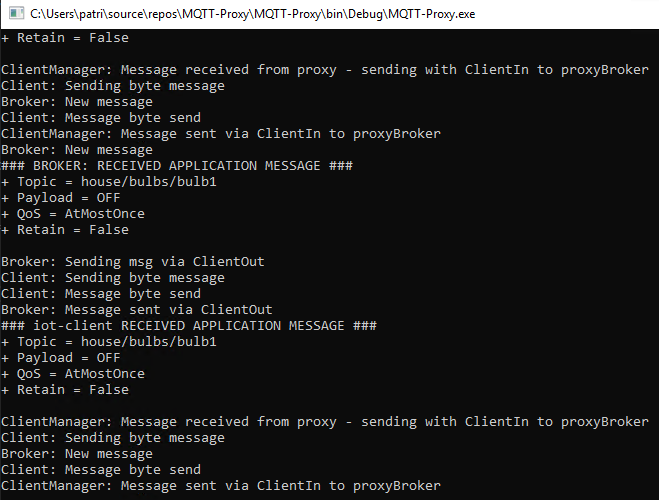
\includegraphics[width=12cm]{tex/bilder/6_validierung/ProxyMessages.png}
    \captionof{figure}{Darstellung der Nachrichten verarbeitet vom Proxy}
    \label{fig:proxy_messages}
\end{figure}

Das Frontend des \emph{Interceptors}, welches auf Abbildung \ref{fig:frontend_messages} zu sehen ist, ist die Kernkomponente der Software. Sie zeigt alle abgefangenen Nachrichten und ermöglicht, diese zu filtern, editieren und erneut zu versenden. Die Nachrichten werden chronologisch untereinander aufgelistet. Pro Nachricht werden dem Nutzer alle wichtigen Inhalte bereitgestellt.
\begin{figure}[!h]%h=direkt danach t=top b=bottom
    \centering
    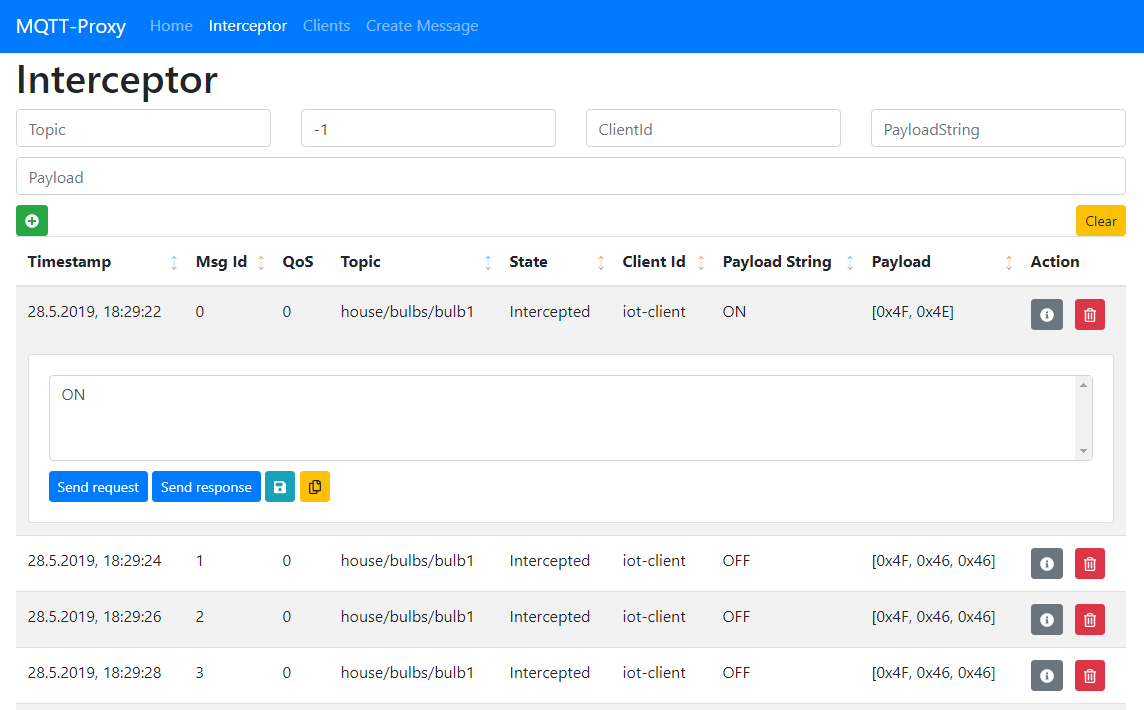
\includegraphics[width=14cm]{tex/bilder/6_validierung/FrontendInterceptor.png}
    \captionof{figure}{Darstellung der Nachrichten im Frontend}
    \label{fig:frontend_messages}
\end{figure}

\section{Performance}
    Hier wird die Performance des Proxys analysiert, um Hinweise auf Skalierbarkeit und zur Ausführung notwendige Ressourcen zu erhalten.
    Folgende Messwerte wurden mithilfe des \emph{Visual Studio Profilers} auf der \ac{VM} des Proxys erfasst.
    
    \begin{enumerate}
        \item Ohne Clients:
        Solange das Programm im Leerlauf arbeitet, also nur Events registriert, die auf Einwirkung anderer Komponenten warten, benötigt es rund 19 \ac{MB} \ac{RAM} und hat eine maximale \ac{CPU} Auslastung von einem Prozent.
        \item Mit einem Client:
        Sobald der erste Client sich verbunden hat, wir nur ein \ac{MB} mehr \ac{RAM} benötigt, in einer Summe von 20 \ac{MB} resultiert. Im Gegensatz dazu werden nun nach der ankommenden Nachricht vom \ac{IoT}-Client alle Funktionen des Programms ausgeführt. Dies führt zu einer Erhöhung beim Ausführen der "Connect"-Funktion auf 20 Prozent und anschießend maximal 17 Prozent.
        \item Mit zwei Clients:
        Kommt nun ein weiterer Client dazu, sodass nun zwei Clients mit dem Proxy verbunden sind, steigt der \ac{RAM}-Verbrauch weiterhin nur um einen Prozent auf 21 \ac{MB} an. Die maximale \ac{CPU} Auslastung steigt jedoch auf 33 Prozent an, was eine Steigerung um 95 Prozent darstellt. Dies ist unter anderem auf ein aktuelles Problem in der Proxy-Implementierung %\cite{https://github.com/Patrick-DE/MQTT-Proxy/issues/3}
        zurückzuführen, das dazu führt, dass jeder Client die Antworten aller Clients an den Proxy schickt. Dies bedeutet, dass Antworten des externen Brokers doppelt erfasst und publiziert werden.
        Bei genauerer Analyse beider am Ansteigen beteiligten Funktionen, ist zu erkennen, dass der größte Ressourcenbedarf bei den folgenden Funktionen zu verorten ist:
        \begin{itemize}
            \item Für 30 Prozent der maximalen \ac{CPU}-Auslastung des Programms ist die "Connect"-Funktion verantwortlich. Die "Connect"-Funktion wird aufgerufen, sobald sich ein \ac{IoT}-Client bei dem Proxy registriert. Sie beinhaltet mehrere kaskadierende Methodenaufrufe, womit der Verbindungsauf von Clients ressourcenintensiv wird.  
            \item Für 57 Prozent der maximalen \ac{CPU}-Auslastung des Programms ist die Systemfunktion \emph{"Console.WriteLine()"} Funktion verantwortlich. Da in diesem Programm viele Informationen an die Konsole zur Information an den Entwickler oder Nutzer weitergereicht werden, ist dies die Hauptursache dafür, dass das Programm die oben genannten \ac{CPU}-Auslastung aufweist. Zu bemerken ist jedoch, dass diese nur den maximalen Wert anzeigen, welcher nur vorhanden ist, wenn Nachrichten an den externen Broker weitergeleitet werden.
        \end{itemize}
    \end{enumerate}
    %TODO Visual Studio Profiler Screenshot von timeline mit marker auf 1 2 3 Clients